\subsection{CPU}

La primera qüestió a plantejar-nos ha estat quin seria el processador meś adient. Per a prendre una decisió de la forma més encertada possible hem cregut oportú elaborar una taula amb diverses possibilitats i comparar les característiques de totes elles, tal com es pot observar a la taula següent:

\begin{table}[H]
    \centering
    \scalebox{0.7}{
\begin{tabular}{c||c|c|c|c|c|c|c|c|c}
    \hline
Processador & \begin{tabular}[c]{@{}c@{}}Freq \\ (GHz)\end{tabular} & \begin{tabular}[c]{@{}c@{}}SIMD \\ (bits)\end{tabular} & \begin{tabular}[c]{@{}c@{}}SIMD \\ units\end{tabular} & Nuclis & Watts & \begin{tabular}[c]{@{}c@{}}Preu \\ (Dòllars)\end{tabular} & \begin{tabular}[c]{@{}c@{}} GFlops/ \\ Socket \end{tabular} & \begin{tabular}[c]{@{}c@{}}GFlops/ \\ Watts\end{tabular} & \begin{tabular}[c]{@{}c@{}}GFlops/ \\ Dòllar\end{tabular} \\ \hline \hline
\rowcolor[HTML]{EFEFEF} 
ThunderX2 CN9980          & 2.20       & 128                                                       & 2                                                        & 32    & 180   & 1795       & 563.20        & 3.13        & 0.314         \\
ThunderX2 CN9978          & 2.20       & 128                                                       & 2                                                        & 30    & 175   & 1600       & 528.00        & 3.02        & 0.330         \\ \hline
\rowcolor[HTML]{EFEFEF} 
AMD EPYC 7702P            & 2.00       & 256                                                       & 2                                                        & 64    & 200   & 4783.99    & 2048.00       & 10.24       & 0.428         \\
AMD EPYC 7502P            & 2.50       & 256                                                       & 2                                                        & 32    & 180   & 2493.99    & 1280.00       & 7.11        & 0.513         \\
\rowcolor[HTML]{EFEFEF} 
AMD EPYC 7742             & 2.25       & 256                                                       & 2                                                        & 64    & 225   & 7581.02    & 2304.00       & 10.24       & 0.304         \\
AMD EPYC 7601             & 2.20       & 256                                                       & 2                                                        & 32    & 180   & 3,388.34   & 1126.40       & 6.26        & 0.332         \\
\rowcolor[HTML]{EFEFEF} 
AMD EPYC 7542             & 2.90       & 256                                                       & 2                                                        & 32    & 225   & 3840.88    & 1484.80       & 6.60        & 0.387         \\ \hline
Intel Xeon Platinum 8253  & 2.20       & 512                                                       & 2                                                        & 16    & 125   & 3115       & 1126.40       & 9.01        & 0.362         \\
\rowcolor[HTML]{EFEFEF} 
Intel Xeon Platinum 8256  & 3.80       & 512                                                       & 2                                                        & 8     & 105   & 7007       & 972.80        & 9.26        & 0.139         \\
Intel Xeon Platinum 8260  & 2.40       & 512                                                       & 2                                                        & 24    & 165   & 4702       & 1843.20       & 11.17       & 0.392         \\
\rowcolor[HTML]{EFEFEF} 
Intel Xeon Platinum 8276  & 2.20       & 512                                                       & 2                                                        & 28    & 165   & 8716       & 1971.20       & 11.95       & 0.226         \\
Intel Xeon Platinum 8280L & 2.70       & 512                                                       & 2                                                        & 28    & 205   & 13012      & 2419.20       & 11.80       & 0.186         \\
\rowcolor[HTML]{EFEFEF} 
Intel Xeon Platinum 8284  & 3.00       & 512                                                       & 2                                                        & 28    & 240   & 15460      & 2688.00       & 11.20       & 0.174         \\ \hline 
\end{tabular}
}
    \caption{Comparativa d'especificacions per cada processador considerat.}
    \label{tab:cpu_cmp}
\end{table}

Per a major precisió i comoditat a l'hora d'analitzar els diversos processadors candidats, els principals criteris valorats per a prendre aquesta elecció, tal com es pot veure a la figura \ref{chartCPUs}, han estat els GFlops/Socket, els GFlops/Watt i els GFlops/Dòllar (sent els GFlops normalitzats respecte la mitjana). 

\begin{figure}[H]
    \centering
    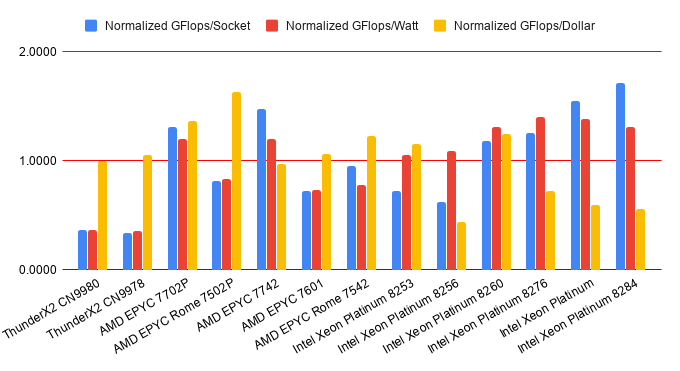
\includegraphics[width=\textwidth]{img/chartCPU}
    \caption{Comparativa entre les diverses CPUs valorades.}
    \label{chartCPUs}
\end{figure}

Després d'estudiar els resultats, per tenir un major marge de maniobre de cara a decisions futures hem pre-seleccionat dos processadors: l'\textit{AMD EPYC 7702P} \cite{cpu_amd_7702_buy} i l'\textit{AMD EPYC Rome 7502P} \cite{cpu_amd_7502_buy}, el primer per mostrar un excel·lent equilibri entre les tres principals característiques estudiades, i el segon per oferir el GFlop més barat sense menystenir excessivament els altres dos aspectes principals.
